
Figure \Cref{fig:resultform} shows First-Order Reliability Method (FORM) results for the 4D truss problem described above. 


\begin{figure}[!htbp]
  \centering {
    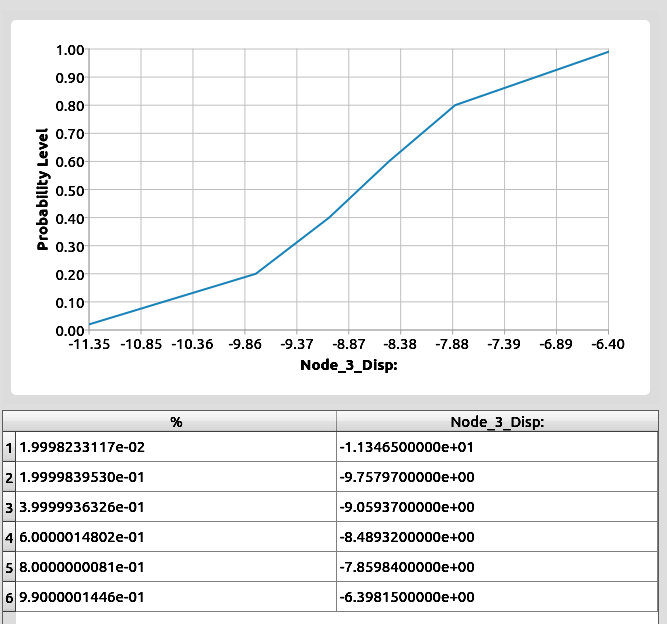
\includegraphics[width=0.8\textwidth]
    {examples/fig_quofem/result_form.png} }
  \caption{First-Order Reliability Method (FORM) results for the 4D truss problem.}
  \label{fig:resultform}
\end{figure}

Figure \Cref{fig:resultgsa} shows the global sensitivity indices for the truss problem at hand, with the main and total sensitivity coefficient for each random variable. 

\begin{figure}[!htbp]
  \centering {
    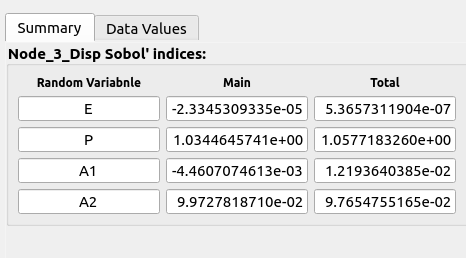
\includegraphics[width=0.8\textwidth]
    {examples/fig_quofem/result_gsa.png} }
  \caption{Main and total global sensitivity indices for the 4D truss problem. }
  \label{fig:resultgsa}
\end{figure}